\chapter{Sound Event Detection}

The task of sound event detection (SED) is defined as the task of analysing a continuous audio stream in order to extract a description of the sound events occurring in it. This description is commonly expressed as a label that marks the start, the ending, and the nature of the occurred sound (e.g., children crying, cutlery, glass jingling). In this chapter two related works are shown, which are respectively: Snoring Sounds Detection by means of Convolutional Recurrent Neural Networks (CRNN) and acoustic data augmentation; and Rare Sound Detection, consisting in detection of three sound categories (i.e., gunshot, babycry and glassbreak) from a highly imbalanced dataset. The latter has been performed by means of a hierarchical framework of ConvNets.

\section{Snoring Sounds Detection}

As described in \secref{sec:snoring_classification}, one of the most common sleep disorder is the chronic snoring. In the occasion of the Interspeech 2017 ComParE challenge \cite{ComParE2017} and subsequent investigations, different approaches based on Deep Neural Networks (DNNs) have been presented \cite{amiriparian2017snore}, \cite{freitag2017end}, \cite{vesperini2018snore} with the aim to classify isolated snore sound events among the four classes based of the VOTE scheme.

In this work, we propose the application of Convolutional Recurrent Neural Networks (CRNNs) to detect snoring episodes from overnight recordings acquired in real life conditions. The method is a two step process: the acoustic spectral features extraction and the CRNN combined with Gated Recurrent Units (GRU) processing. The algorithm is evaluated by using the Average Precision (AP) score.
Differently from other deep learning approaches \cite{amiriparian2017snore}, \cite{freitag2017end}, \cite{vesperini2018snore}, this choice offers a viable and natural solution for jointly learning the spatio-temporal dependencies of audio sequence for discovering snoring event. Additionally, we deal with the high unbalanced setting which exists in the task of snore detection. The original snore/background ratio in the aforementioned signals has been increased by adding isolated snore events from the Munich-Passau Snore Sound Corpus dataset \cite{ComParE2017} (cf. \secref{ssection:MPSSCdataset}). The reliability of the proposed approach is investigated using the A3-snore dataset, leading to significant improvement in term of Average Precision (AP) with respect to Convolutional Neural Network (up to 9.48\%) and other data augmentation techniques.


\subsection{Proposed Approach}

The two step of the proposed approach are detailed in this section, starting from the spectral features extraction and ending with the Convolutional Recurrent Neural Network.

\begin{figure}[t]
	\centering
	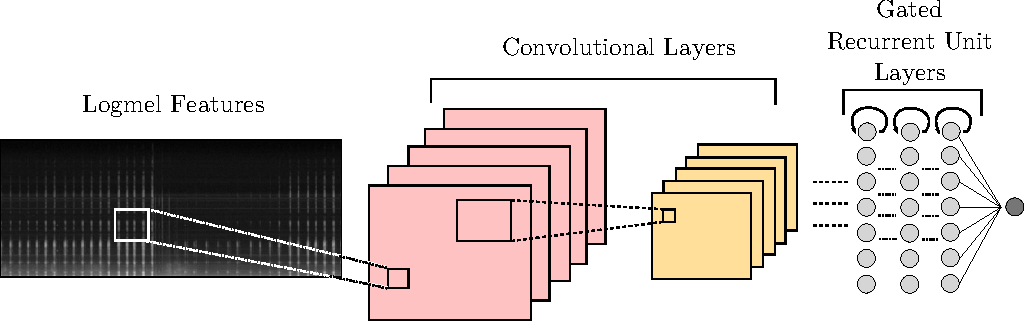
\includegraphics[width=0.9\columnwidth]{img/snore_detection_4.pdf}
	\caption[Proposed approach for Snoring Detection]{The proposed approach scheme for Snoring Detection.}
	\label{fig:overall}
\end{figure}

\subsubsection{Features Extraction}
The feature extraction stage operates on stereo audio signals sampled at 44.1 kHz. 
Following the results obtained in recent works related to sound event detection \cite{DCASE2017Workshop}, we use the log Mel energy coefficients (Logmel) as an efficient representation of the audio signal. The stereo signal is firstly down-mixed to mono by averaging the two channels. 
The resulting audio signal is split into 30\,ms frames and a frame step of 10\,ms, then the Logmel coefficients are obtained by filtering the power spectrogram of the frame by means of a mel filter-bank, then applying a logarithmic  transformation to each sub-band energy in order to match the human perception of loudness. We used a filter bank with 40 mel scaled channels, obtaining 40 coefficients/frame. 

\subsubsection{Convolutional Recurrent Neural Networks}


CRNNs used in this work are composed of four types of layers: convolutional layers, pooling layers, recurrent layers and detection layer. 
Each convolutional layer is followed by batch normalization per feature map \cite{ioffe2015batch}, a leaky rectified linear unit activation function (LeakyReLU) and a dropout layer \cite{srivastava2014dropout} with rate equal to $0.3$.
A frequency domain max-pooling layer is then applied to the resulting feature-map, in order to enhance the relevant information from frequency bands without lose the temporal resolution of the Logmels, as proposed in \cite{cakirconvolutional}. The extracted features over the CNN feature maps are stacked along the frequency axis. Max-Pooling operation combined with shared weight in convolutional layers provide robustness to frequency shifts in the input features and this is crucial to overcome the problem of intra-class acoustic variability for snore events.
In the recurrent block, the stacked features resulting from the last pooling layer are fed to layers composed of GRUs (cf. \secref{sssec:GRU}), where tanh and hard sigmoid activation functions are used for update and reset gates, respectively.
Fast response to the changes in the input and the previous activation information is fundamental for high performance in the proposed algorithm, where the task is to detect a small chunk of consecutive time frames where the target event is present. In addition, a previous work \cite{valenti2017neural} demonstrates improvements provided by recurrent architectures in the sound event detection in real-life audio.
The detection layer is a feed-forward layer of composed of a single neuron with sigmoid activation function, corresponding to the probability the event onset. The layer is time distributed, this means that while computing the output of the classification layer, the same weight and bias values are used over the recurrent layer outputs for each frame.

In a comparative aim, we implemented also a CNN architecture very similar to the CRNN, the only difference being that the recurrent layers of the CRNN are replaced with time distributed feed-forward layers with ReLU activations. In following section, we will refer it as CNN.


The neural networks training was accomplished by the AdaDelta stochastic gradient based optimisation algorithm \cite{zeiler2012adadelta} for a maximum of 500 epochs on the binary cross entropy loss function. The optimizer hyperparameters were set according to \cite{zeiler2012adadelta} (i.e., initial learning rate $lr=1.0$, $\rho=0.95$, $\epsilon=10^{-6}$). An early stopping strategy, monitoring the validation AP score, was employed in order to reduce the computational burden and avoid overfitting. 


\subsection{A3 Snore Dataset} 

The snore detection algorithm has been evaluated on the A3-Snore dataset. A brief description of the acquisition setup and dataset splitting is provided in the following.

\subsubsection{Acquisition setup:}
In order to capture the overnight audio recordings a ZOOM-H1 Handy Recorder has been used. It is equipped with two unidirectional microphones set at a 90 degree angle relative to one another. The signals are stored in WAV files with a sampling rate of 44.1\ kHz and bit depth equal to 16.
The input gain is automatically set by the recorder to prevent overload and distortion, while the high-pass filter was enabled in order to eliminate pops, wind noise, blowing, and other kinds of low frequency rumble.


\subsubsection{Acquisition environment:}
The acquisition environment consist of a simple bedroom, with two access points (door and window). The recorder is placed near the patient, at same height of the bed and in line with the subject's mouth. During the recordings, the patient is the only one that can occupy the bedroom, in order to avoid contaminations on recorded audio signals. The room dimensions are reported in \figref{fig:room}.
Background sounds include traffic noise, breathing and speech signals, house and animal noises. We acquired some samples measurements of the event-to-background (EBR) ratios considering background noise, snoring events and noise events such as ``car passing by'' or ``dog barfing''. The EBR resulted equal to 6.5 dB and 1.1 dB respectively for noise to background EBR and snore to background EBR. 


\begin{figure}[t]
	\centering
	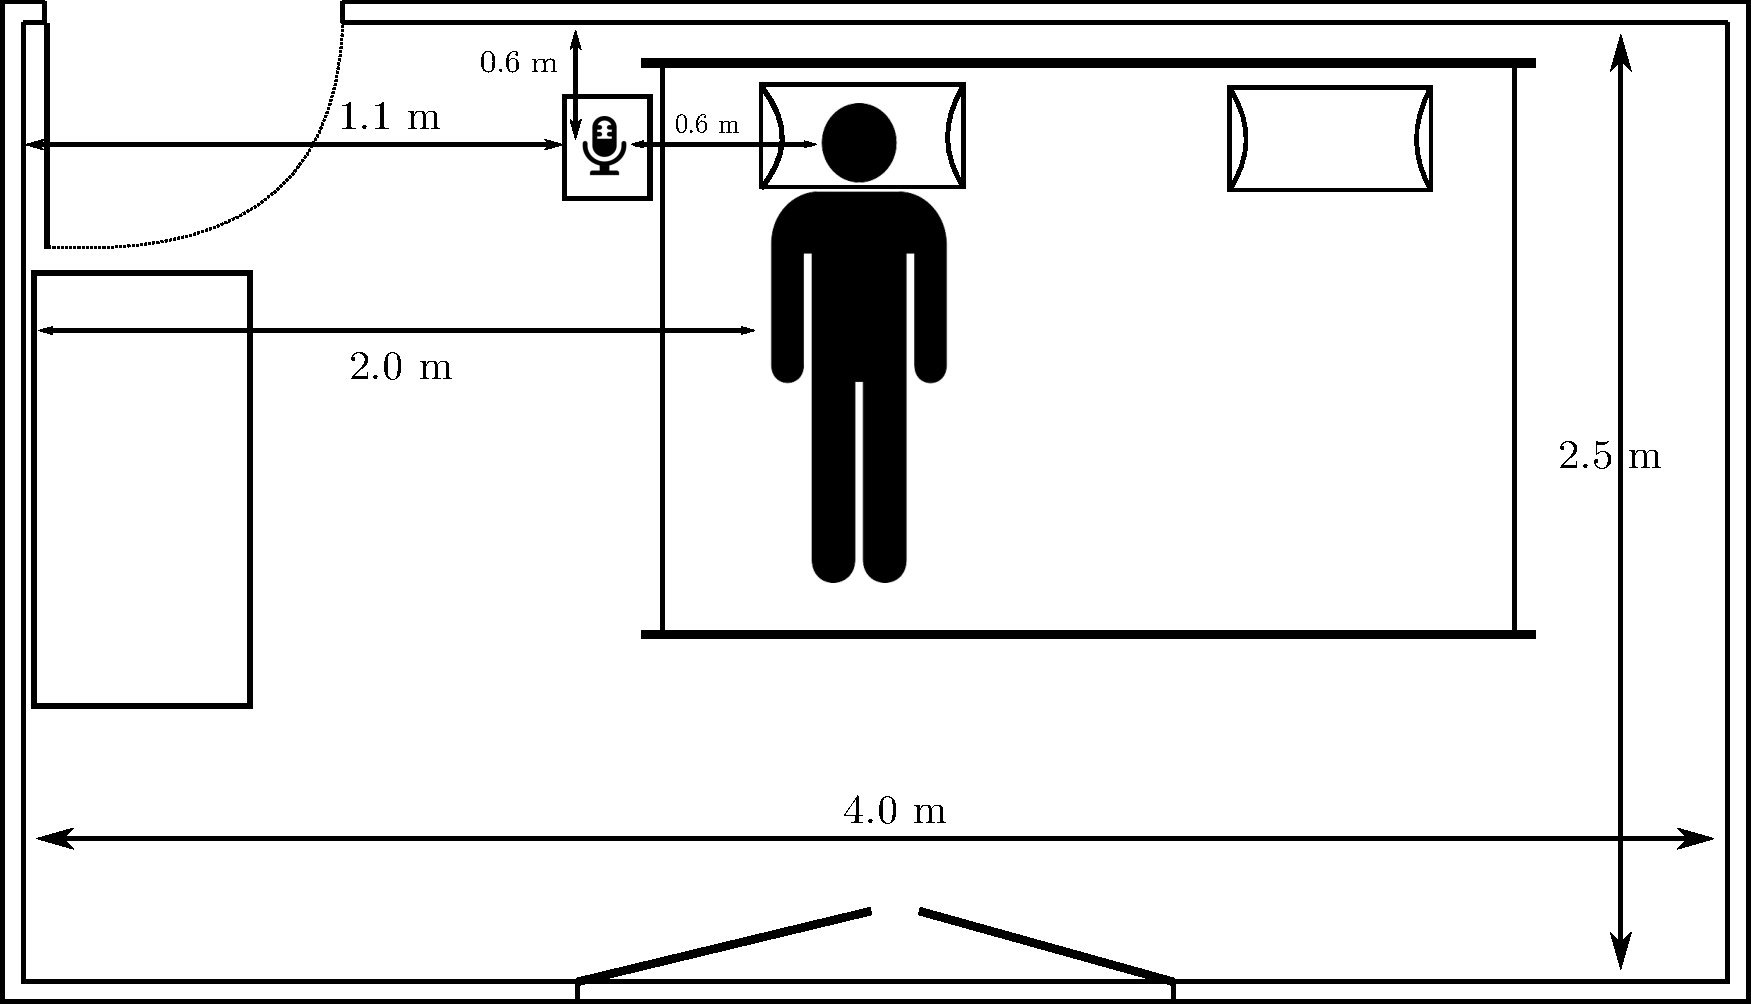
\includegraphics[width=0.6\columnwidth]{img/room.pdf}
	\caption{Plant of the recording room.} 
	\label{fig:room}
\end{figure}


\subsubsection{Dataset splitting:}
The original recordings have been manually labelled, annotating the snore events onset and offset with a resolution of 1 second. The audio sequences have been divided into chunks of 10 minutes, and only those with the highest number of snore events have been used in the experiments. 
The dataset is organized into subjects, which can be respectively used as \emph{training} or \emph{validation} sets in a two fold cross validation strategy (i.e., Leave One Subject Out procedure). The number of events per class in the database is strongly unbalanced as reported in \tableref{a3snore}. Thus, the snore detection task is challenging, due to the high number of noises on the A3-SNORE dataset. 

\begin{table}[ht]
	\centering
	\resizebox{\textwidth}{!}{
	\begin{tabular}{cccccc}
		\hline
		\multicolumn{6}{c}{\textbf{A3-SNORE dataset}} \\
		\hline
		\# & Gender & Age & Snoring (SN) & Total Duration (Tot) & Ratio (SN/Tot) \\
		\hline
		Snorer 1 & M & 48 & 33m-27s & 3h-12m-0s & 14.5\% \\
		Snorer 2 & M & 55 & 21m-21s & 3h-50m-0s & 11.1\% \\
		\hline
		\multicolumn{3}{l}{Total} &	54m-48s	& 7h-02m-0s	& 12.8\%\\
		\hline    
	\end{tabular}
	}	
	\caption[A3-SNORE dataset]{Difference of recording times for each class, divided by snorers.}
	\label{a3snore} 
\end{table}

\subsection{Data Augmentation Techniques}
\label{ssec:data-augmentation}
In this application, what we are really interested is to detect the minority class (e.g. snoring events) rather than the majority class (e.g. background). Thus, we need to adequately train the models in order to obtain a fairly high prediction for the minority class. In order to counteract the dataset unbalancing existing in the task of snoring detection different techniques of data augmentation have been evaluated. 
The literature suggests that it is possible to augment training data in data-space or in feature-space. 
In this work, both data augmentation approach have been evaluated, by using the \emph{Synthetic Minority Over-sampling Technique} (SMOTE) \cite{chawla2002smote} in the feature space, and by generating simulated data with an increased number of snore events. 
The original snore/background ratio in the acquired signals has been increased with these transformations to approximately 30\% \cite{young1997nasal}, maintaining anyway a natural unbalance which is properly of this task.
In the following sub-sections, a brief description of each method is provided.

\subsubsection{Majority Class under sampling:} it is not a properly data augmentation technique but it is a fast and easy way to balance the data. It consists in randomly selecting a subset of data from the training sets in order to modify the ratio of the sample occurrences in two classes.

\subsubsection{SMOTE:} It is an over-sampling approach in which the minority class is over-sampled by creating new synthetic examples. The minority class is over-sampled by taking each minority class sample and introducing synthetic examples along the line segments joining any/all of the \emph{k} minority class nearest neighbors (\emph{k}-NN). Depending upon the amount of required over-sampling, neighbors from the \emph{k}-NNs are randomly chosen. In particular, synthetic samples are generated in the following way: the difference between the feature vector (sample) under consideration and its nearest neighbor is multiplied by a random number between $0$ and $1$, and this is added to the feature vector under consideration. In details, for a sample $x_{i}$:
\begin{equation}
x_{j}^{\text{SMOTE}} = x_{i} + (\tilde{x}_{i,k} - x_{i}) \cdot r(j)
\end{equation}
where $r(j) \in [0,1]$.
This causes the selection of a random point along the line segment between two specific features. This approach effectively forces the decision region of the minority class to become more general. 

\subsubsection{Proposed approach - Generating simulated data:} The simulated training sets have been created starting from the folds described in \secref{ssec:dataset}.
The impulse responses between the snore source and the microphones have been recreated by using the library Pyroomacoustics \cite{Scheibler2018}.
Isolated snore sounds have been taken from the Munich-Passau Snore Sound Corpus (MPSSC) dataset \cite{ComParE2017}. It is composed of 843 snore events which have been extracted and manually screened by medical experts from Drug-Induced Sleep Endoscopy (DISE) examinations of 224 subjects.
The augmented training set has been created by convolving the isolated snore sound events of the MPSSC corpus with the synthetic impulse responses. Than, the obtained signals have been mixed with the original recordings without overlap with the already present events. The artificial added event dynamic was normalized to the maximum value observed in the original signals. The resulting total time of snore signals is 55 minutes for Snorer 1, and 56 minutes and 5 seconds for Snorer 2.

\subsection{Experimental Setup}
The performance of the algorithms has been evaluated in term of AP score, a metric that summarizes the Precision and Recall curve (cf. \secref{sec:evaluation_metrics}).
To asses the performance of the models, we explored different hyper-parameter configurations and, for each of these, we repeated the whole experiments training the models both with the original data and  with  data processed with techniques described in \secref{ssec:data-augmentation}. \tableref{CNN-params} shows the hyper-parameter configurations analyzed in our experiments. They regard kernels size, kernel number and GRUs for a total of 120 experiments. In the case of CNN the number of units and layer refers to a Multi Layer Perceptron (MLP) architecture. The experiments were conducted in a 2-fold cross-validation strategy corresponding on a leave one subject out procedure, thus in fold 1 we used Snorer 1 as training set and Snorer 2 as validation set and in fold 2 vice-versa. The models were selected on the performance based on the AP score  averaged on the two folds. 
The algorithm has been implemented in the Python language using Keras \cite{chollet2015keras} as deep learning library. All the experiments were performed on a computer equipped with a 6-core Intel i7, 32\,GB of RAM and two Nvidia Titan X graphic cards. 

\begin{table}[ht]
	\centering
	\begin{tabular}{|l|r|}
		%		\hline
		%		\multicolumn{2}{|c|}{Network Layout Parameters}            \\ \hline
		\hline
		Convolutional Layers Number & 3                            \\ \hline
		Kernel Number               & 4, 8, 16, 32, 64                 \\ \hline
		Kernel Size                 & $5\times5$, $3\times3$, $2\times2$ \\ \hline
		Pooling Size                & $5\times1$, $4\times1$, $2\times1$ \\ \hline
		\hline
		Recurrent Layers Number     & 2, 3                            \\ \hline
		Dense Layers Number     & 2, 3                            \\ \hline
		Number Of Units             & 4, 8, 16, 32, 64                 \\ \hline
	\end{tabular}
	\caption[Snoring Detection - Experiments]{Explored network layout parameters.}
	\label{CNN-params}
\end{table}


\subsection{Results}
The performance of the CRNN and CNN architectures using different data augmentation techniques are reported in \figref{fig:results}. In blue are depicted results with CRNN, in green the results of the CNNs. The CRNNs show to be effective for snore event detection yet with the original data, although the dataset imbalance. The best performing model is composed of 3 CNN layers with respectively [64,64,64] filters of size $3\times3$ and two GRU layers of 64 units. This configuration obtains an AP up to 82.05\%, with a difference of +7.79\% with respect to the CNN.

\begin{figure}[h]
	\centering
	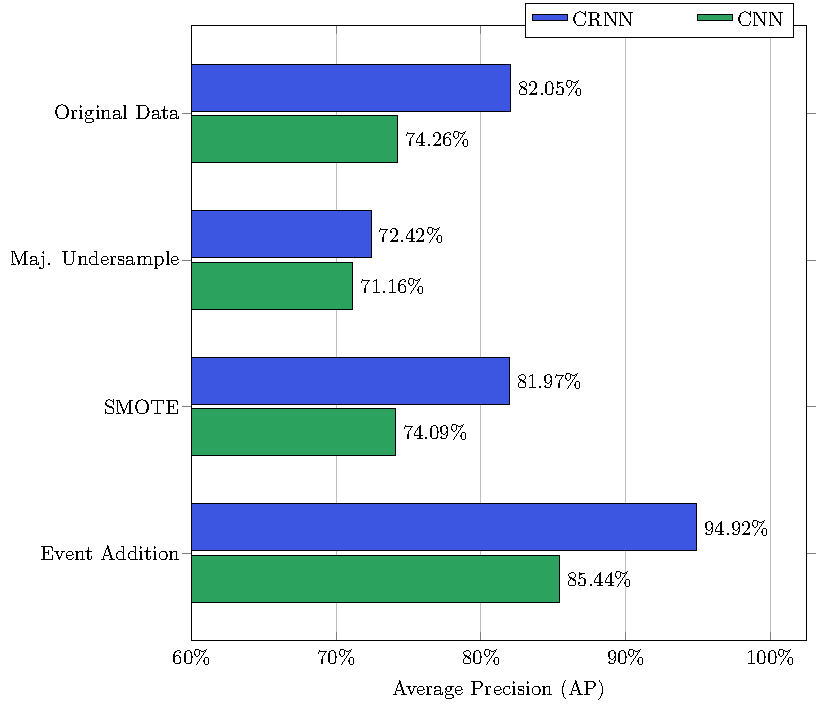
\includegraphics[width=0.7\columnwidth]{img/grafTex/results.pdf}
	\caption[Snoring Detection - Results]{Results with different data augmentation techniques for the best models of the evaluated architectures.} 
	\label{fig:results}
\end{figure}

The majority class under-sampling and the SMOTE techniques obtain worst performance with respect to original recordings. For majority class under sampling this can be motived by the necessity of DNN models of a large amount of data to be trained properly, thus a reduction of data samples cannot benefits to their detection ability. Regarding the SMOTE, the performance reduction is less dramatic (-0.16\% and -0.08\%, respectively, for CNNs and CRNNs) but its employment remains vain. In this case, the motivation can be found on the complexity to generate new samples of audio signals in the feature space which can really improve a DNN perfomance.

The addition of isolated snore samples convolved with the simulated room impulse response has a tangible beneficial effect on the examined models. In fact, with this technique we obtain an AP improvement equal to 11.18\% and 12.87\%, respectively, for the CNN and the CRNN. The latter obtains an AP equal to 94.92\% with an architecture composed of 3 CNN layers with respectively [64,32,32] filters of size $5\times5$ and two GRU layers of 32 units.
This model is composed of 91,553 free-parameters and occupies approximately 1.2 MB, providing to the algorithm a feasible complexity in an application scenario.


\subsection{Conclusion}
In this work, a deep learning algorithm based on a CRNN architecture fed with Logmel spectral features extracted from the audio signal has been proposed for snore detection. The A3-Snore dataset has been acquired in real-world conditions, containing overnight recordings of two male subjects and it has been used to assess the performance of the models. The original snore/background ratio has been increased by adding isolated snore events from the Munich-Passau Snore Sound Corpus dataset \cite{ComParE2017}. The reliability of the proposed approach has been investigated with respect to baseline CNN and different data augmentation techniques such as oversampling (i.e., SMOTE) and downsampling. Results show that the presented snore detection methodology is able to better generalize across different users. In particular, the CRNN is able to extract salient information from the spectral features in order to discriminate snore events, while the implemented data augmentation provide additional samples of the minority class (i.e., snore events). These samples contains supplementary information that can be exploited by the CRNN for learning and discriminate snore events.
Future works will be addressed to employ this methodology in a weakly supervised setting.
Specifically, in the real-life applications, the precise annotation of existing events from overnight recordings can be onerous and can be result in sparse labeling. Machine learning models trained in a weakly supervised fashion can help to counteract this problem without losing the state of the art performance.

\newpage
%%%%%%%%%%%%%%%%%%%%%%%%%%%%%%%%%%%%%%%%%%%%%%%%%%%%%%%%%%%%%%%%%%%%%%%%%%%%%%%%%%%%%%%%%%%%%%%%%%%%%%%%%%%%%%%%%%%%%%%%%%%%%%%%%%%

\section{Rare Sound Event Detection}

The ``Detection of rare sound events'' task of the 2017 Detection and Classification of Acoustic Scenes and Events (DCASE) challenge \cite{DCASE2017Workshop} consisted in determining the presence and the precise onset time of three types of sounds, ``baby cry'', ``glass break'' and ``gun shot'' in artificially generated audio sequences. 
The task takes into account real-world issues that introduce additional complexity to the problem, such as the acoustic variability of the sounds belonging to each event class, the presence of environmental noise and its variability, etc. The rules of the challenge allow to know \textit{a priori} the event typology possibly present in the audio sequence under examination, thus it is possible to have a separate binary classifier for each class.

\subsection{Related Works}
In the recent era of the ``Deep Learning'' different approaches to SED have been proposed marking use of the capabilities of deep neural networks (DNNs) to learn the relation between time-frequency features of the raw audio signal and a target vector representing sound events.
Although the DNNs based systems are more computationally intensive with respect to  widely used statistical modelling methods such as hidden Markov models (HMMs) or Gaussian mixture models (GMMs)  \cite{heittola2010audio, peng2009healthcare}, a comparative study \cite{sigtia2016automatic} has highlighted that they are able to achieve top performance in the sound recognition problem.

A well-fitting example of such performance is given in~\cite{marchi2017deep}, where different DNNs are trained on three datasets recorded in real life environments in order to detect abnormal events or hazardous situations exploiting only the information carried by the acoustic signal. The experimental results show that Deep Recurrent Neural Networks (DRNNs) outperform the probabilistic approaches over the three databases. 
Another example focuses on employing Convolutional Neural Networks (CNN)  for Voice Activity Detection in multi-room domestic scenarios (mVAD) \cite{vecchiotti2018convolutional}. The CNN-mVAD results to be effective and outperforms the other method with a significant solidity in terms of performance statistics.

In occasion of the DCASE 2017 challenge, many novel systems featuring deep neural networks have been proposed, in particular involving hybrid architectures making use of Convolutional Neural Networks (CNN) and DRNNs. In detail, both the first two classified algorithms make use of mel spectrogram coefficients as spectral representation of the audio signal which is processed by a CNN with 1D filters in the case of the first ranked \cite{limrare} or by a 2D CNN with frequency pooling in the case of the second classified \cite{cakirconvolutional}. The architectures are, then, combined with recurrent layers to process the features obtained by the convolutional blocks.
In \cite{phan2017dnn} the authors propose a hierarchical structure based on CNNs and DNNs trained with multi-task loss functions. Specifically, in the first stage the networks are trained for background noise rejection, using a weighted loss function to penalize the false positive errors. In the second stage the multi-task loss enables the networks to simultaneously perform the event classification task and the onset time estimation. This approach obtained the third place in the final ranking. 
All of the aforementioned systems largely outperform the baseline system based on a Multi Layer Perceptron architecture (MLP) and Logmel energies as features.
The baseline system \cite{DCASE2017challenge} is based on a Multi Layer Perceptron architecture (MLP) and log mel energies as features. For each audio frame, the input vector is constructed concatenating 5 adjacent log mel vectors for a total of 200 elements. The ANN architecture consists of two dense layers of 50 hidden units each and one output neuron with sigmoid activation, which indicates the activity of the target class.

\subsection{Proposed Method}
The proposed system is a hierarchical algorithm composed of five stages: the acoustic features extraction, the event detection stage 1,  which produces an output at frame-rate and a dedicated smoothing procedure of this signal.
Then, a refinement of the previous decision stage is performed by a 2D CNN which discards possible false positives detected by the stage 1. The final decision procedure annotates the effective onset time of the active event. In \figref{fig:flow-chart-rare-sed} the phases of the algorithm are depicted. This is an extended and improved method with respect to our contribution to the DCASE 2017 \cite{vesperinihierarchic}.

\begin{figure}[t]
	\centering
	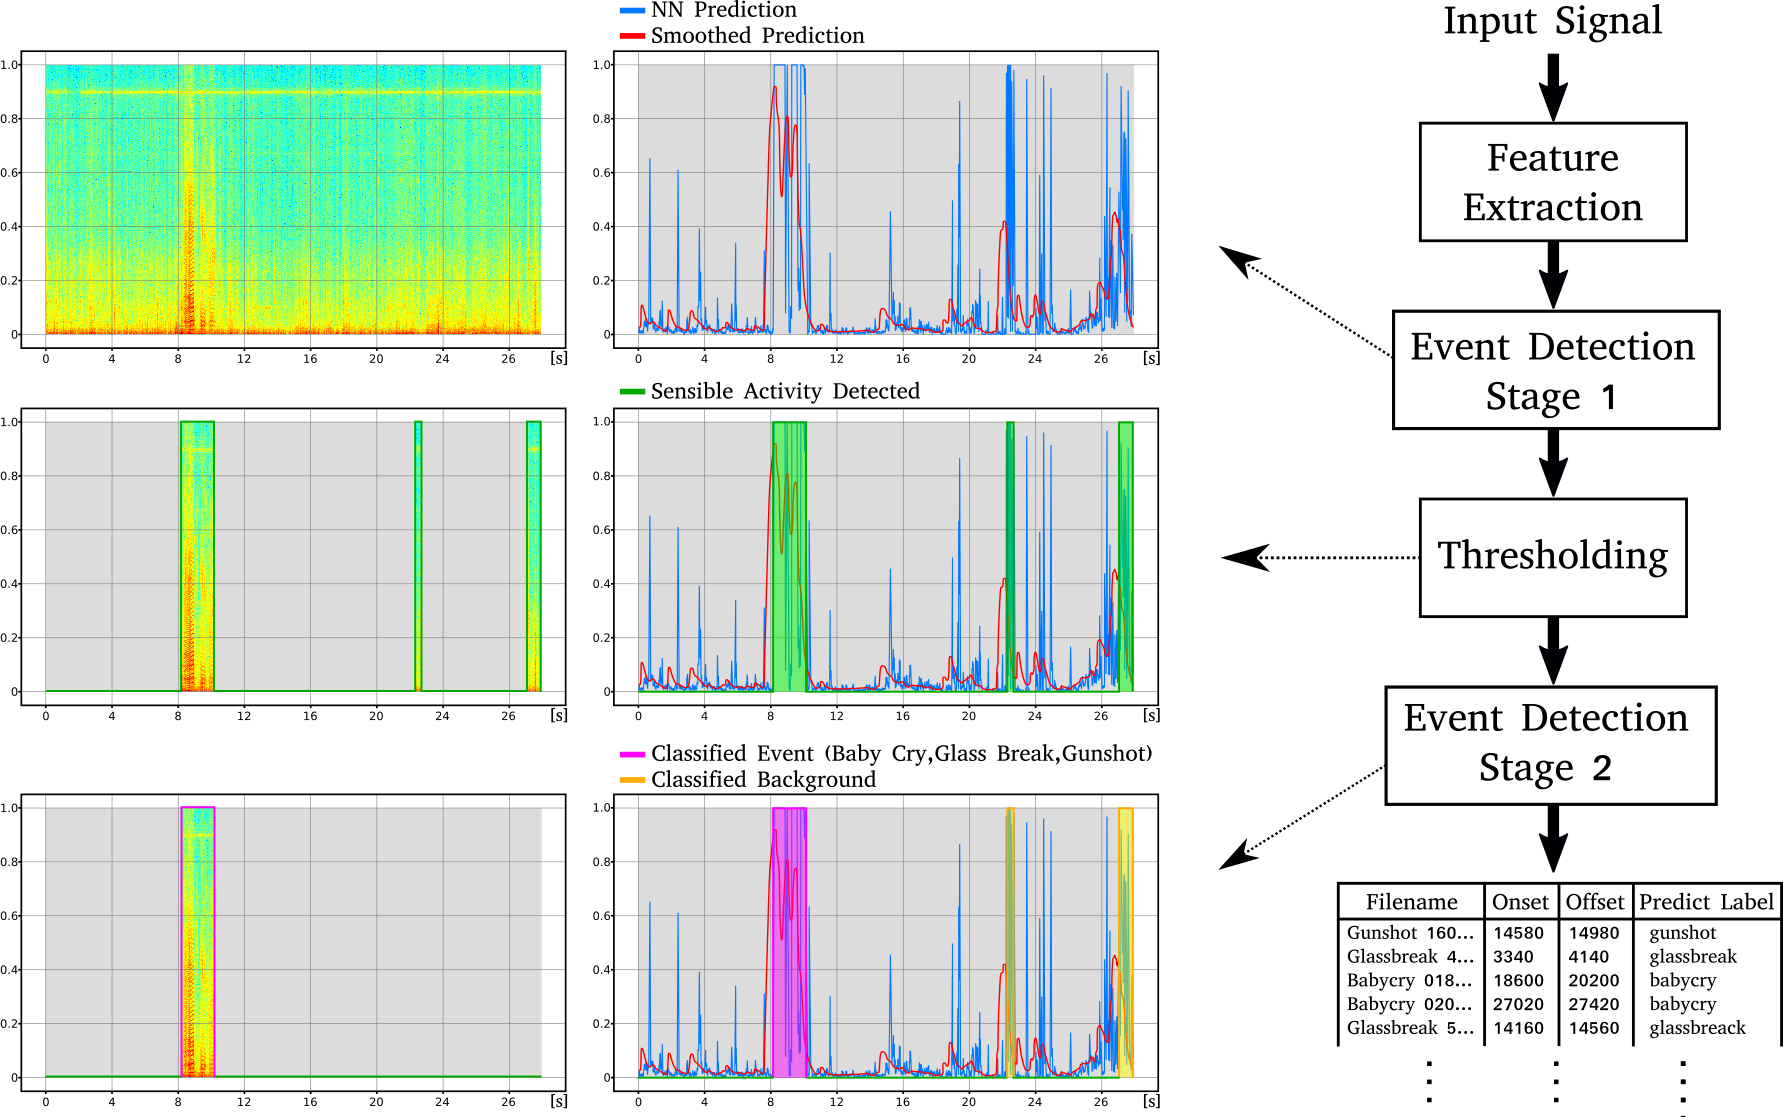
\includegraphics[width=0.9\columnwidth]{img/approccio_finale_1.png}
	\caption[Proposed approach for Rare Sound Event Detection]{Flow chart of the proposed method for rare sound event detection. Each event class implements such a scheme. In the first column are shown the spectrograms of the input signal and of the detected events. In the second column the network outputs at each stage of the algorithm.}
	\label{fig:flow-chart-rare-sed}
\end{figure}

\subsubsection{Features Extraction}
The feature extraction stage operates on mono audio signals sampled at 44.1 kHz. 
Following the results obtained at the DCASE2017 challenge by \cite{cakirconvolutional}, we use the log mel energy coefficients (Logmel) as an efficient representation of the audio signal. In addition, we explored the combination of the Logmel with features based on wavelet coefficients and forward prediction errors (WC-LPE) \cite{marchi2014multi}. A brief description of the features extraction procedures is given below.
\paragraph{Logmel coefficients}
The audio signal is split into frames of 40\,ms and a frame step of 20\,ms, then the Logmel coefficients are obtained by filtering the power spectrogram of the frame by means of a mel filter-bank, then applying a logarithmic  transformation to each sub-band energy in order to match the human perception of loudness. We used a filter bank with 40 mel scaled channels, obtaining 40 coefficients/frame. 

\paragraph{WC-LPE Feature}
The Wavelet Coefficient (WC) and Linear Prediction Error (LPE) feature set relies on non-stationary signal components and it has been successfully exploited for musical note onset detection \cite{marchi2014multi}. WC-LPE extraction is done by first processing the input signal with a Discrete Wavelet Transform (DWT) dyadic tree. Then, each DWT sub-band is filtered by a linear prediction error filter (LPEF), obtaining Forward Prediction Errors (FPE). All LPEF outputs and DWT sub-bands are resampled to an intermediate sampling rate and rectified. The feature set is, finally, created from the DWT sub-bands, their first order time derivatives, the FPE and their first order time derivatives.

For both feature sets the range values of each coefficient is normalized independently according to the mean and the standard deviation computed on the training sets of the neural networks.

\subsubsection{Event Detection Stage 1}
The Event detection (ED) stage 1 has the goal to discard frames containing only background sounds, reducing as much as possible the false negative decisions.
We evaluated two DNN architectures as binary classifiers: the MLP and the CNN with 2D kernels and frequency pooling. In both cases, the output layer is formed by two units with the \textit{softmax} non-linear function. Thus, the networks outputs represent the probabilities that an input feature vector $\mathbf{x}[t]$ at the frame index $t$ belongs to the background or the event class. In our analysis, we evaluated as network input the Logmel coefficients and the combination of the latter with the WC-LPE features.

\subsubsection{Deep Neural Network Architectures}
For the ED stage 1 we compared the performance of two deep neural networks architecture, respectively the Multi Layer Perceptron (MLP) and the Convolutional Neural Networks (CNN). In both cases, the neural networks training was accomplished by the AdaDelta stochastic gradient-based optimisation algorithm \cite{zeiler2012adadelta} for a maximum of 500 epochs on the binary cross entropy loss function. The optimizer hyperparameters were set according to \cite{zeiler2012adadelta} (i.e., initial learning rate $lr=1.0$, $\rho=0.95$, $\epsilon=10^{-6}$). An early stopping strategy monitoring the validation loss was employed in order to reduce the computational burden. Thus if the validation loss does not decrease for 20 consecutive epochs, the training is stopped and the last saved model is selected as the final model. In addition, dropout is used as regularization technique \cite{srivastava2014dropout} with rate $0.5$. 

\paragraph{Multi Layer Perceptron Neural Network}
The network is designed to consider a temporal context  $C$, thus the network input  feature vector  $\hat{\mathbf{x}}[t]$ is obtained concatenating $\mathbf{x}[t]$ with the previous $\mathbf{x}[t - c]$, with $c = 1, \dots, C$. 
 
During the training procedure, additive zero-centered Gaussian noise with $\sigma=0.1$ was applied to $\hat{\mathbf{x}}[t]$ as a form of data augmentation, improving the generalization capabilities of the DNN and avoiding overfitting \cite{marchi2017deep}.


\paragraph{Convolutional Neural Network}
\label{ssec:CNN}

In our case the convolutional layer input is a matrix $\mathbf{X} \in \mathbb{R}^{F \times T}$, where $F$ and $T$ represent respectively and the number of Logmel channels and the number of frames of the acoustic signal.
When we combine the two aforementioned feature sets, we process them with two separate sets of convolutional layers, gathering two feature maps that are concatenated along the feature axis. Before concatenation, batch normalization \cite{ioffe2015batch} is applied to each feature map and a leaky rectified linear unit activation function (LeakyReLU) with $\alpha=0.3$, followed by a feature domain max-pooling layer.
Finally, fully connected layers are stacked, applying the same weights and biases to each frame element. The output layer for each of the binary classifier neural networks has two neurons corresponding to the probability of the background or the event onset. We can discard, thus, one of the two neurons without loss of information, and we will consider the output of the neuron corresponding to the event activation $u[t] = y_{t,2}$, as the output of the network at frame $t$.


\subsubsection{Post Processing}
In the post processing stage, each network output is convolved with an exponential decay window of length $M$ defined as:
\begin{equation}
	\mathbf{w}[t]= e^{-\frac{t}{\tau}} \quad \text{with}  \, \tau =  \frac{-(M-1)}{log_e(0.01)}
\end{equation}
The result is processed with a sliding median filter with local window-size $k$. Finally, a decision threshold $\theta$ is applied.

\subsubsection{Event Detection Stage 2}

The aim of the event detection stage 2 is to eliminate false positives, by removing the events wrongly detected at the previous stage. This is done by feeding a binary-classifier CNN with chunks of features in correspondence to the detected events (colored region in the bottom right spectrogram of \figref{fig:flow-chart-rare-sed}). At this stage only Logmel coefficients are used as input features, in order to reduce the computational burden of the model. Non-overlapping feature matrices $\mathbf{X}$ of size $F\times20$ are used during training, while 95\%-overlapping feature matrices are employed during testing (1-frame shift).
A chunk size of 20 corresponds to 0.4 seconds of audio, i.e. half the minimum possible length of the occurring events, leading to an analysis of the audio event at different time and frequency resolutions with respect to previous stages. The ED Stage 2 NN is trained for 100 epochs on the binary cross entropy loss function with the AdaDelta gradient descent algorithm.


\subsubsection{Final Decision}

For each audio sequence, we perform a classification on contiguous blocks of frames detected as event by the ED stage 1. Among contiguous frame chunks classified as ``event'' by the CNN, the first frame with highest network output is indicated as event onset.


\subsection{Experimental Set-Up}

According to the DCASE 2017 guidelines, the performance of the proposed algorithm has been assessed by using the development dataset for training and validation of the system. Furthermore, a blind test on the provided evaluation dataset has been performed.
The performance metric of the DCASE 2017 challenge is the event-based error rate (ER) calculated using onset-only condition with a collar of 500 ms. The algorithm has been implemented in the Python language using Keras \cite{chollet2015keras} as deep learning library. All the experiments were performed on a computer equipped with a 6-core Intel i7, 32\,GB of RAM and two Nvidia Titan X graphic cards.

\subsubsection{Dataset}
The DCASE2017 challenge dataset \cite{DCASE2017challenge} has been used to develop and evaluate the algorithm.  The dataset consists of 30-second long sequences of background acoustic scenes recorded in different public or domestic spaces (park, home, street, cafe, train etc.) \cite{mesaros2016tut}, some of which have been added with isolated recordings from at most one of the three different target sound event classes: baby crying, glass breaking and gun shot. 
The presence probability of a sound event in each mixed sequence of the original Development set was 0.5, thus we kept only sequences containing a sound event of the original training set and we generated additional mixtures assigned to the training and the validation sets.
For the development set a total number of sequences respectively equal to 2750 for training, 300 for validation and 1496 for test have been employed.
This change increases the percentage of the frames including a target event in the training data, which helps to ease the problem of data imbalance. In addition, due to the fast decay of the ``gun shot'' sound, we generated more sequences containing this event class compared to the others, in order to maintain approximately the same percentage between frames containing event samples and backgrounds.

In the evaluation set, the training and test sequences of the development set are combined into a single training set,  while the validation set is the same used in the Development dataset. The system is evaluated against an ``unseen'' set of 1500 samples (500 for each target class) with a sound event presence probability for each class equal to 0.5.


\subsubsection{First Event Detection Stage}


\begin{table}[b]
	
	\centering
	\footnotesize
	\begin{tabular} {|c | c | c|}
		\hline
		Parameter & Range & Distribution\\  
		\hline
		\hline                                     
		MLP layers Nr.  & [2 - 7]& uniform \\
		\hline                                     
		MLP layers dim. & [20 - 4048]& log-unifom \\
		\hline                                     
		MLP Context & [1 - 7] & uniform\\
		\hline
		Activation & [tanh - relu] & uniform\\
		\hline
	\end{tabular}
	\caption[Rare Sound Event Detection - ED Stage 1 Experiments]{Hyper-parameters optimized in the random-search phase for the MLP ED stage 1, and their range.}
	\label{tbl:hyper-params-mlp}
\end{table}


\begin{table*}[t]	
	\centering
	\footnotesize
	\resizebox{\textwidth}{!}{
	\begin{tabular}{l|c|c|c|c|c|c|c|c|}
		\cline{2-9}
		& \multicolumn{4}{c|}{\textbf{Development Dataset}}          & \multicolumn{4}{c|}{\textbf{Evaluation Dataset}}                 \\ \hline
		\multicolumn{1}{|l|}{Features}         & Babycry & Glassbreak & Gunshot & \textbf{Average} & Babycry & Glassbreak & Gunshot & \textbf{Average} \\ \hline
		\multicolumn{9}{|c|}{\textbf{MLP ED Stage 1 }}                                                                                                          \\ \hline
		\multicolumn{1}{|l|}{Logmel}         & 0.19    & 0.12       & 0.16    & \textbf{0.16}    & 0.64    & 0.54       & 0.58    & 0.59             \\ \hline
		\multicolumn{1}{|l|}{Logmel + WC-LPE} & 0.23    & 0.10       & 0.19    & 0.17             & 0.76   & 0.55       & 0.55    & 0.62             \\ \hline
		\multicolumn{9}{|c|}{\textbf{CNN ED Stage 1}}                                                                                                          \\ \hline
		\multicolumn{1}{|l|}{Logmel}         & 0.23    & 0.13       & 0.18    & 0.18             & 0.48    & 0.23       & 0.44    & 0.38             \\ \hline
		\multicolumn{1}{|l|}{\textbf{Logmel + WC-LPE}} & 0.25    & 0.09       & 0.16    & 0.17             & 0.46    & 0.10       & 0.36    & \textbf{0.31}    \\ \hline
		\hline
		\multicolumn{9}{|c|}{\textbf{MLP ED Stage 1 + CNN ED Stage 2}}                                                                                       \\ \hline
		\multicolumn{1}{|l|}{Logmel}         & 0.14    & 0.08       & 0.16    & \textbf{0.13}    & 0.31    & 0.25       & 0.44    & 0.33             \\ \hline
		\multicolumn{1}{|l|}{Logmel + WC-LPE} & 0.20    & 0.09       & 0.19    & 0.16             & 0.37    & 0.27       & 0.40    & 0.35             \\ \hline
		\multicolumn{9}{|c|}{\textbf{CNN ED Stage 1 + CNN ED Stage 2}}                                                                                        \\ \hline
		\multicolumn{1}{|l|}{Logmel}         & 0.19    & 0.10       & 0.16    & 0.15             & 0.31    & 0.17       & 0.39    & 0.29             \\ \hline
		\multicolumn{1}{|l|}{\textbf{Logmel + WC-LPE}} & 0.18    & 0.08       & 0.17    & 0.14             & 0.25    & 0.10       & 0.31    & \textbf{0.22}    \\ \hline
	\end{tabular}
	}
	\caption[Rare Sound Event Detection - Results]{Results in terms of ER score for all the evaluated combination of proposed ANNs and features used in Event Detection Stage 1.}
	\label{tab:results_edstage1}
\end{table*}


To assess the performance of the MLP employed in the event detection stage 1 we resorted to a random search strategy \cite{bergstra2012random}.
Table \ref{tbl:hyper-params-mlp} shows the parameters explored in the random search, as well as the prior distribution and ranges. We evaluated 300 sets of layout parameters (100 for each event class) repeated for the two input features combination.

Regarding the CNNs, we explored the hyper-parameters space by means of a grid search for a total of 75 experiments (25 for each event class) covering the number of convolutional filters per layer $\{16,32,64\}$, the kernels shape $\{3 \times 3, 5 \times 5\}$, the number of MLP layers $\{1,2,3\}$ and their respective number of units $\{16,32,64,128\}$. The feature
max-pool sizes after each convolutional layer were $\{5,4,2\}$ for all the explored layouts. Also in this case the experiments were repeated for both the input features combination.

A successive grid search was performed for each network configuration evaluated, in order to find the post-processing parameters that yielded the minimum error rate. Investigated parameters in the grid search were: exponential window length $w$ in the range $\{10,20,\dots,90\}$, median filter kernel $k$ in the range $\{9,11,\dots,31\}$ and threshold $\theta$ in the range $\{0,0.05,\dots,0.5\}$. 

Once the best models on the Development dataset were found, a fine tuning of the post processing parameters was done during the validation stage, in order to assess the performance of the whole system. In fact, the hierarchical architecture of the algorithm allows to set a lower threshold in the first decision stage in order to reduce the deletions at the expenses of some insertions. These will be removed by the ED stage 2. 



\paragraph{Training set for CNN based ED Stage 2 }
To compose the dataset for training and evaluation of the CNNs dedicated to each target audio event we proceeded as follows: the samples of each event class were selected between the audio sections respectively labelled as ``baby cry'', ``glass break'' and ``gun shot'' from the mixtures of the DCASE 2017 development dataset, in addition with the isolated events source signals. To obtain the background samples, we processed with the first stage of our algorithm sequences from the same dataset which do not contain events. 
Thus, the frames detected as event in this case represent the ``false positive'' or ``insertions'' of the stage 1. 
We used those frames as background samples in the CNN training phase to improve its event classification abilities and balancing the dataset. 

\subsubsection{Refinement Stage}
To design the best refinement CNN model for our purposes, we generated a shuffle stratified validation split from the dataset composed as described above. We left out the 30\% of the samples as validation set for the CNN model and we selected the layout parameters of the neural network based on the F-measure score obtained on this data sub-set. 
The best performing model was the same for all the target audio events and was composed as follows: three convolutional layers with $\{32,32,32\}$ filters, respectively, of size $5\times5$. The convolutional layers were followed by a feature max pooling layer with kernels of size $\{5,4,2\}$, respectively. Three dense layers composed of 32 neurons with $tanh$ activation functions were applied before the network output layer, for a total number of network parameters equal to 35K. 


\subsection{Results}
Results reported in Table \ref{tab:results_edstage1} are obtained as follows: we selected the models with lowest ER for each combination of DNN architecture and input features operating in the ED stage 1 and we evaluated the systems separately for each target class before the ED stage 2 on the Evaluation set, keeping ED stage 1 post processing parameters fixed. Then, with the same settings we obtained the performance of the whole system both on Development and Evaluation datasets. The architecture composed of a first stage with 2D CNN fed by Logmel and WC-LPE features resulted the best performing on the Evaluation dataset, obtaining an average ER equal to 0.17.
Details of these architectures are reported in Table \ref{tab:CNN_details}.


\begin{table}[b]
	\centering	
		\begin{tabular}{|l|c|c|c|}
			\hline
			Hyper-parameters & Babycry                            & Glassbreak                         & Gunshot                            \\ \hline
			Conv. Kernels    & 5$\times$5, 3$\times$3, 3$\times$3 & 3$\times$3, 3$\times$3, 3$\times$3 & 3$\times$3, 3$\times$3, 3$\times$3 \\
			Kernel shape     & 32, 16, 16                         & 64, 64, 64                         & 32, 16, 16                         \\
			MLP Layers size  & 32, 32                             & 128, 128                           & 32, 32                             \\ \hline
			\# Parameters    & 18k                            & 185k                           & 17k                           \\ \hline
		\end{tabular}
	\caption[[Rare Sound Event Detection - ED Stage 1 Best models]{Details of models for CNN based ED stage 1 with the lowest ER on Development set. All of them use a combination of log mel energies and WC-LPE as input features.}
	\label{tab:CNN_details}
\end{table}
The experimental results show how this combination improves generalization properties of the algorithm. In fact, the MLP based stage 1 with only Logmel features obtains the best overall ER equal to 0.13 on the Development dataset, but the performance decreases significantly on the Evaluation set. In addition, the number of free parameters of the best performing MLP models was always an order of magnitude greater w.r.t. the CNN models. Regarding the stage 2, its beneficial effect is supported especially with the Evaluation dataset: in this case, the improvement in terms of ER given by the joint detection procedure is evident and it gives additional robustness to the system in terms of generalization.

In Table \ref{tab:params} the overall results between best ranked systems of the DCASE 2017 Challenge are compared. It can be observed that the best two scores have been obtained with ensemble methods, involving the additional computational cost of running several architectures in parallel, while the table reports the number of parameters per architecture. Although the proposed system does not outperform the first two methods, the average number of network parameters is significantly lower. This provides greater scalability in real-world applications.

\begin{table}[t]
	\centering
	\begin{tabular}{|l|c|c|}
		\hline
		Approach        & Evaluation ER & \# Parameters \\ \hline
		Lim et al. \cite{limrare}      & \textbf{0.13}                               & 6200K          \\ 
		Cakir et al.  \cite{cakirconvolutional}   & 0.17                               & 756K          \\ 
		Proposed system & 0.22                               & \textbf{108K}         \\ 
		Phan et al. \cite{phan2017dnn}   & 0.27                               & 2100K          \\ \hline
	\end{tabular}
	\caption[Rare Sound Event Detection - Comparative Results]{Comparison between the obtained ER scores and the number of parameters with the first three ranked approaches at the DCASE2017 Challenge.}
	\label{tab:params}
\end{table}


\subsection{Conclusion}
In this paper, a framework that makes use of hierarchical CNN classifiers fed with Logmel and WC-LPE features has been proposed for rare SED, providing significantly improved performance over the baseline system for every target sound event class in DCASE 2017 challenge dataset. The system also provides a significant reduction of the network parameters w.r.t. other competitive algorithms.  
The multi-scaled approach inherent to the two different CNN architectures results to be effective. 

For future work, strategies to customize the loss function embedding the evaluation metric into the training procedure can be considered. Specifically, this task is particularly affected by the dataset unbalancing: to counteract this problem an alternative to the data augmentation is to design tailored loss functions which enhance the detection of the rare events. 

%%%%%%%%%%%%%%%%%%%%%%%%%%%%%%%%%%%%%%%%%%%%%%%%%%%%%%%%%%%%%%%%%%%%%%%%%%%%%%%%%%%%%%%%%%%%%%%%%%%%%%%%